\documentclass[10pt,a4paper]{article}
\usepackage[utf8]{inputenc} % para poder usar tildes en archivos UTF-8
\usepackage[spanish]{babel} % para que comandos como \today den el resultado en castellano
\usepackage{a4wide} % márgenes un poco más anchos que lo usual
\usepackage[parfill]{parskip}
\usepackage{mathtools}
\usepackage{enumitem}
\usepackage[margin=50pt]{geometry}
\usepackage{amsfonts}
\usepackage{flafter}
\usepackage{listings}
\lstset{
numbers=left,
numbersep=15pt,
}


\begin{document}
\setlength{\parindent}{8pt} %sangria

\section{Ejercicio 1}

\subsection{Introducción}
\noindent \underline{\textbf{Contexto}}

Estamos encarando una competencia, en la que dados distintos puentes colgantes y participantes, estos deben cruzar los puentes sin caerse, dado que bajo cada puente corre un río de lava hirviendo.
Estos puentes tienen una característica importante, y es que no todos sus tablones están en óptimas condiciones, estando algunos rotos, y haciendo que si alguien los pisa, caiga sin remedio hasta el río de lava que fluye debajo. Esta es la única forma de caer del puente. Afortunadamente, estos tablones rotos se encuentran marcados, de forma que quien este cruzando el puente, sepa si puede pisar o no un tablón.
Un requisito de la competencia es que los puentes solo pueden ser cruzados dando saltos, tanto para ingresar o salir del puente como para avanzar de tablón en tablón.
En cuanto a los participantes, debido a su estado físico, cada uno tiene una capacidad máxima de tablones que pueden cruzar de un solo salto.
Notar que si hay demasiados tablones rotos consecutivos, si un participante no tiene la capacidad suficiente de salto para cruzarlos a todos juntos, entonces ese participante no podrá cruzar el puente ya que indefectiblemente caerá si lo intenta.
El ganador de la competencia será quien haya cruzado todos los puentes, dando la menor cantidad de saltos.

\noindent \underline{\textbf{El problema a resolver}}

Debemos diseñar un algoritmo, que dado un participante, la capacidad máxima de tablones que puede cruzar de un solo salto (salto máximo), un puente, con un número n de tablones del mismo y un mapeo de los tablones rotos, indique si es posible cruzar el puente y de ser así, indique a qué tablones debería saltar para cruzarlo dando la menor cantidad de saltos posibles. El algoritmo deberá tener complejidad O(n), siendo n la cantidad total de tablones (rotos y no rotos) del puente colgante.
En el caso en el que el participante no pueda cruzar el puente, debe devolverse la palabra "no".
Así mismo, el programa debe soportar resolver muchas instancias de este tipo ingresadas.

\noindent \underline{\textbf{Ejemplos}}

\noindent Para los ejemplos denotaremos:

\textit{C}, a la cantidad de tablones que el participante en cuestion puede cruzar de un solo salto.\newline
\indent \textit{N}, a la cantidad de tablones (rotos y no rotos) del puente en cuestion, donde a cada tablon los enumeraremos entre 1 y N.

\begin{enumerate}[leftmargin=0.5cm]

\item C = 4, N = 8, donde los tablones rotos son: 1,3,6,8.

El algoritmo debería devolver: 3 4 7 9

\item C = 4, N = 17, donde los tablones rotos son el 2,3,4,5.

El algoritmo debería devolver: no, puesto que una vez en el tablón 1, el participante no puede pisar ningún tablón que su capacidad C le permite pisar.

\item  C = 5, N = 41, donde no hay tablones rotos.
                         
El algoritmo debería devolver: 9 5 10 15 29 25 39 35 40 42

\end{enumerate}
\newpage

\subsection{Desarrollo}

Como idea principal para la resolución del problema, partiremos de la siguiente propiedad del problema:
para cualquier tablón $\boldsymbol{n_0}$ en que se esté situado en un momento dado, hacer un salto de distancia \textbf{X}, es siempre mejor que un salto de distancia \textbf{J}, para todo \textbf{J\textless X}. Este razonamiento 'goloso' es válido ya que vale que luego de saltar hasta x, se puede saltar a todos los que se podría haber saltado desde j, y posiblemente, más aún.

Es decir, si notamos CS[i], donde 0\textless i$\leq$n, (con n = cantidad de tablones del puente), como la conveniencia de salto para un tablón i, vale que:

\textbf{(}$\boldsymbol\forall$ \textbf{j,x:nat, j\textless x) CS[j]} $\boldsymbol\leq$ \textbf{CS[x]}

Por lo dicho anteriormente, concluimos (y en el siguiente inciso, demostraremos) que saltar a la posición más lejana posible dentro del rango de salto k (propio del jugador), nunca sera peor que hacerlo a una posición anterior a ésta y más aún, será la óptima decisión.

Con el siguiente pseudocódigo explicamos las bases principales de nuestro algoritmo:

\noindent Sea \textbf{S} el salto m\'aximo posible.\\
Sea \textbf{C} la cantidad de tablones del puente pasado como par\'ametro (tablones v\'alidos y no v\'alidos).\\
Sea \textbf{saltos} el vector en el que se almacenar\'an las posiciones a las que se salte. Cuando se declara a este vector, se le reserva un tama\~no \textbf{C}, ya que a lo sumo pueden realizarse \textbf{C} saltos (uno por tabl\'on).\\
Sea \textbf{actual} última posición válida a la que se saltó.\\
Sea \textbf{tablon\_en\_revision} el tabl\'on que estoy revisando en el ciclo.\\

\begin{lstlisting}
	Si (S > C) // Caso 1
		agrego C+1 a Saltos
		encontre solucion y salgo
	Si no // Caso 2
		si (S < 1)	
			no hay solucion y salgo
	Si no // Caso 3
		para (i entre 0 y C)
			actualizo el tablon_en_revision
			si (i es posicion valida)
				actualizo salto_mas_largo_posible
			si (tablon_en_revision - actual == S)
				actualizo actual
				agrego actual a saltos
			si (actual + S > C)
				agrego C+1 a saltos
				encontre solucion y salgo

\end{lstlisting}

\noindent En el condicional de la línea 1, se chequea si el rango de salto S pasado como parámetro supera a la cantidad de tablones, es decir, si con un solo salto se puede recorrer todo el puente. Si ese es el caso, se sale del algoritmo.\\
En el condicional de la línea 2, se chequea si no hay rango de salto S, en ese caso, el problema no tiene solución.\\
En el último condicional (línea 7), se entra a un ciclo en el que se van a recorrer del 0 al C (sin incluir) todos los tablones, llevando un registro del tablón que se esta revisando en la i-ésima iteración (lo llamamos tablon\_en\_revision), así como también, cuál es la última posición válida hacia la que salté (en el pseudocódigo la llamaremos actual). Si tablon\_en\_revision es válido, se lo guarda como potencial candidato a salto, dado que, hasta el momento, es el salto más largo posible. Luego, se chequea si, dada la posición actual y el tablon en revisión, ya chequee todos los tablones a los que potencialmente podía acceder desde actual (línea 12), sí es así, debo guardar como salto realizado al potencial candidato a salto (en el pseudocódigo lo llamamos salto\_mas\_largo\_posible) en el vector en el que almaceno los saltos y luego, actualizar como actual a esta posición, ya que se convertirá en la última posición válida hacia la que salté. Por último, verificamos si con el próximo salto desde la posición actual se llegará a cruzar el resto del puente, es decir, si al dar mi próximo salto encontré la salida (línea 15). Si ese es el caso, agrego la posición de salida (la C+1) y salgo del ciclo.\\
Finalmente, devolvemos el vector de saltos y su tamaño como solución del problema, en el formato pedido.\\
Vale la pena mencionar que repetiremos este algoritmo una vez por cada instancia pasada como entrada.\\



\subsection{Correctitud}

Sea \textbf{P} un puente pasado como par\'ametro y \textbf{C} la cantidad de tablones del mismo, describiremos \textbf{Z}, una soluci\'on del problema, como el arreglo que contiene un máximo C de elementos x donde $\forall$ x $\in$ Z, P[x] = 0, es decir, es una posici\'on v\'alida a la que el participante salt\'o (tambi\'en nos referiremos a estas posiciones como a los "saltos").
Demostraremos la siguiente propiedad, llam\'emosla M:\\

\textbf{M} = para cualquier \textbf{a} tabl\'on v\'alido de un puente P, con a $\in$ \{1\,...\,n\} y un salto m\'aximo k que un jugador puede realizar, efectuar el salto desde a hacia p = max\{a\,...\,a+k\} (siendo p una posici\'on v\'alida del puente) genera una menor o igual cantidad de saltos en Z que cualquier otra posici\'on distinta de p elegida.\\

Esto es equivalente a afirmar que cumpliendo la propiedad \textbf{M}, una solución es \'optima para el problema planteado, es decir, $\vert$M(Z)$\vert$ $\leq$ $\vert$Z$\vert$. Esto es: la longitud de Z  \underline{si para Z vale la propiedad M} \textbf{es menor o igual} a la longitud de Z en otras condiciones. (Aclaraci\'on: por longitud nos referimos a la cantidad de saltos realizados) \\

Supongamos una solución \textbf{S} óptima, donde hay algún \textbf{a} para el cual no vale \textbf{M}, es decir, se escoge una opción de salto \textbf{Q} $\neq$ max\{a\,...\,a+k\}, donde \textbf{Q} es una posición válida.\\
Consideremos entonces ahora a \textbf{S'}, una solución para la misma instancia que posee hasta la posición \textbf{a} los mismos saltos, pero que en \textbf{a}, en vez de realizar un salto a \textbf{Q} se realizó un salto a la posición válida \textbf{P} = max\{a\,...\,a+k\}.\\
Llamaremos $R_{p}$ al rango de posiciones válidas accesibles desde \textbf{P} $\in$ \{P\,...\,P+k\} y $R_{q}$ al \textbf{S} al rango de posiciones válidas accesibles desde \textbf{Q} $\in$ \{Q\,...\,Q+k\}.\\
Sabemos que $R_{p}$ $\cap$ $R_{q}$ $\neq$ $\emptyset$ ya que por lo menos exite \textbf{P} que es posición válida que es accesible desde $R_{q}$ y pertenece a $R_{p}$, ya que \textbf{Q} $<$ \textbf{P} $\leq$ \textbf{Q+k} $\leq$ \textbf{P+k}.

	\begin{figure}[h]
		\begin{center}
		   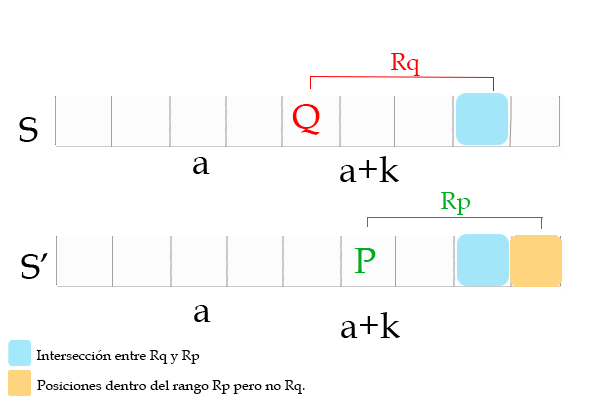
\includegraphics[scale=0.50]{esquema.png}
		\end{center}
	\end{figure}

Entonces pueden darse los siguientes casos:\\

(a) Existe al menos un \textbf{x} tal que \textbf{x} no pertenece a $R_{p}$ $\cap$ $R_{q}$ y x $\in$ $R_{p}$, es decir, existe una posición que es accesible desde \textbf{P} pero no desde \textbf{Q}. Acceder a esta posición solo puede provocar que se generen en total menos o igual cantidad de saltos que en \textbf{S}, ya que, en caso de ser necesario acceder a estas posiciones, desde \textbf{S} se debería haber realizado un salto extra, en cambio en \textbf{S'}, estas posiciones son accesibles en el primer salto \textbf{P}.
En el caso de que no sea necesario accederlas, se mantendría la misma cantidad de saltos que en \textbf{S}, por lo que \textbf{S'} sería igualmente óptima.\\

(b)En el caso de que no exista \textbf{x} tal que \textbf{x} no pertenece a $R_{p}$ $\cap$ $R_{q}$ y \textbf{x} $\in$ $R_{p}$, $R_{p}$ contiene las posiciones válidas entre \{P\,...\,Q+k\}, por lo que como teníamos \textbf{Q} $<$ \textbf{P} $\leq$ \textbf{Q+k}, se sigue que $R_{p}$ esta incluído en $R_{q}$, entonces obtendremos la misma cantidad de saltos en \textbf{S'} que en \textbf{S}, ya que en \textbf{S}, desde \textbf{P} el próximo salto válido será \textbf{Q+k}, que era el próximo salto válido desde \textbf{Q} en \textbf{S}. De esta forma, mantengo igualada la cantidad de saltos: de \textbf{a} a \textbf{Q} y de \textbf{Q} a \textbf{Q+k} en \textbf{S} y de \textbf{a} a \textbf{P} y de \textbf{P} a \textbf{Q+k} en \textbf{S'}.

Quedan así verificados todos los casos, demostrándose que una solución que cumple con la propiedad \textbf{M} es óptima.\newpage

%%%%%%%%%%%%%%%%%%%%%%%%%%


%%%%%%%%%%%%%%%%%%%%%%%%%%%%%%%%%%%%%%%%%%%%

\subsection{Complejidad}
\noindent Sea \textbf{S} el salto m\'aximo posible.\\
Sea \textbf{C} la cantidad de tablones del puente pasado como par\'ametro (tablones v\'alidos y no v\'alidos).\\
Sea \textbf{saltos} el vector en el que se almacenar\'an las posiciones a las que se salte. Cuando se declara a este vector, se le reserva un tama\~no \textbf{C}, ya que a lo sumo pueden realizarse \textbf{C} saltos (uno por tabl\'on).\\
Sea \textbf{actual} última posición válida a la que se saltó.\\
Sea \textbf{tablon\_en\_revision} el tabl\'on que estoy revisando en el ciclo.\\

\begin{lstlisting}
	Si (S > C) // Caso 1
		agrego C+1 a Saltos
		encontre solucion y salgo
	Si no // Caso 2
		si (S < 1)	
			no hay solucion y salgo
	Si no // Caso 3
		para (i entre 0 y C)
			actualizo el tablon_en_revision
			si (i es posicion valida)
				actualizo salto_mas_largo_posible
			si (tablon_en_revision - actual == S)
				actualizo actual
				agrego actual a saltos
			si (actual + S > C)
				agrego C+1 a saltos
				encontre solucion y salgo

\end{lstlisting}

\noindent Dependiendo de los par\'ametros de entrada S y C se entrar\'a por el Caso 1, Caso 2 o Caso 3 (notemos que entrar se puede entrar por un y solo un caso).\\
Tanto el Caso 1 como el 2 se basan en operaciones elementales que se ejecutan una cantidad constante de veces, por lo tanto, en ambos casos la complejidad es O(1).\\
En el Caso 3 tenemos como operaci\'on principal un ciclo for que se ejecuta a lo sumo C veces (puede llegar a ejecutarse menos de C veces si en alguna de las iteraciones, por el condicional de la l\'inea 15, se sale del ciclo).\\
Luego, tenemos todas operaciones elementales, sea cual sea el caso de que valga cualquier combinaci\'on posible de los condicionales de las l\'ineas 10, 12 o 15.\\
Finalmente, el Caso 3 tiene complejidad (en peor caso) de C operaciones elementales, es decir, C*O(1). Entonces, la complejidad temporal del Caso 3 es O(C).\\
Podemos ver entonces que la complejidad temporal del algoritmo termina siendo:\\
\begin{itemize}
\item[•]O(1) si se entra por el Caso 1 o 2.
\item[•]O(C) si se entra por el Caso 3.\\
\end{itemize}
Por lo anterior, en peor caso, la complejidad temporal del algoritmo propuesto es O(C).\newpage

%\thispagestyle{empty}
\subsection{Experimentación}
\noindent Para el proceso de experimentación del problema se plantearon distintos escenarios de test para corroborar que el algoritmo propuesto funcionara correctamente y que la cota de complejidad encontrada y justificada en la sección anterior, en la práctica, se cumpliera.\\

\noindent Llamamos escenario de test a un conjunto de pruebas que si bien son distintas, comparten alguna similitud.\\

\noindent Por ejemplo, un escenario es aquel en el cual un participante puede dar saltos de una distancia k constante, y las distintas pruebas del escenario variarían en el tamaño del puente y en el estado de sus tablones.\\

\noindent Dado que el CPU de la computadora utilizada para tomar los tiempos no está atendiendo únicamente a nuestro proceso, realizar una sola vez cada prueba podría darnos valores que no son cercanos a los reales. Para minimizar este margen de error, a cada prueba de cada escenario se la hizo ejecutar un total de 10.000 veces y se tomó el mejor valor. Notar que tomar el mejor valor no es una mala decisión, ya que mientras más chico sea el valor, más cerca estamos del valor real de tiempo que toma el algoritmo para una instancia dada.\\

\noindent En cada prueba se tomaron métricas para la posterior evaluación del algoritmo en la práctica. Notar que la medición no contempla tiempos de entrada/salida de datos, sino que contempla solamente el núcleo del algoritmo.\\

\noindent Para cada escenario testeado, se hicieron gráficos 2D que permitan ver de una manera más clara los resultados obtenidos en las pruebas del mismo. Estos fueron realizados con el software QitPlot que la cátedra proveyó.\\

\noindent En cuanto a qué casos testear, decidimos testear los casos “border” y casos aleatorios, mezclando en todos los casos distintas variaciones de saltos posibles, tamaño de los puentes y estado de los tablones de los mismos.\\

\noindent Los casos "border", son aquellos que están en los extremos de las capacidades del algoritmo, es decir, el mejor caso que el algoritmo puede resolver, y el peor. 
Para las instancias aleatorias, se diseñó un generador de estas, que dada una longitud, el estado de generaría los tablones se haría de forma aleatoria, es decir, dado un tablón t, en una prueba t puede ser válido y en otra no.  Este generador es capaz de generar múltiples instancias aleatorias.
Para todos los casos, se eligió una precisión de hasta 0,0001 ms (milisegundos). De ser menor, la notamos como 0.\\

\noindent En todos los casos se pudo comprobar que la práctica refleja lo expuesto en incisos anteriores.

\newpage \subsubsection{Escenario de mejor caso del algoritmo}

\noindent Para el algoritmo propuesto, el mejor caso de respuesta es el caso en el que la capacidad de salto del participante es superior a la longitud del puente, este caso tiene una complejidad de orden constante, es decir, el mejor caso es O(1).

\noindent Notar que para probar el mejor caso, la capacidad de salto no puede ser un parámetro variable, ya que es necesario que sea mayor que la cantidad de tablones.

\noindent Para evaluar el mejor caso, el generador de instancias, aplica como salto máximo, el tamaño del puente + 1. Por ende, para cada prueba realizada, si el puente contenía n tablones, el salto era de n+1.
Dicho esto, se generaron distintas instancias del algoritmo, con distintos tamaños, y con puentes de estado aleatorios, para verificar que el mejor caso no del estado de sus tablones, sino de que el salto sea mayor estricto que la cantidad de tablones.

\noindent Luego de realizar las pruebas pertinentes de este escenario, (y de realizar  10.000 veces cada una) como declaramos al inicio del insiso, mostramos los resultados obtenidos en el siguiente gráfico:

	\begin{figure}[h]
		\begin{center}
		   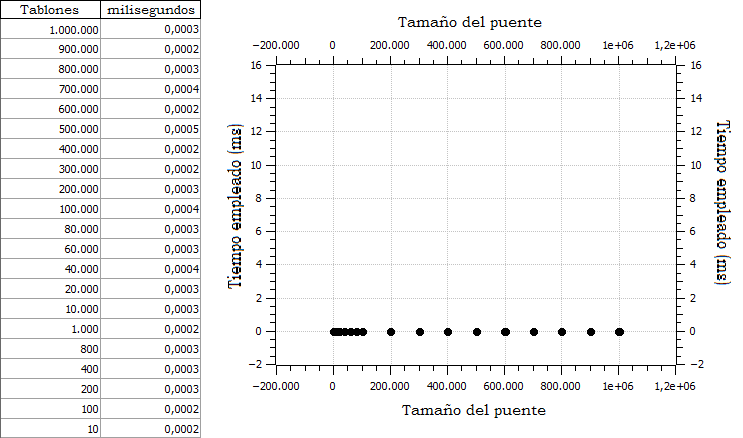
\includegraphics[scale=0.75]{casosDeTest/GRAFICOS/png/Ej1mejorCasoPNG.png}
		\end{center}
	\end{figure}

\indent En la figura superior se puede apreciar que el tiempo de resolución es constante a pesar de variar el tamaño de entrada y el estado de los tablones (generados aleatoriamente).\\

\subsubsection{Escenario de peor caso del algoritmo}

\noindent Para el algoritmo propuesto, el peor caso de respuesta, es decir, el caso que más tiempo demanda ejecutar,  es aquel en el que el participante puede cruzar todo el puente (por lo que el algoritmo debe continuar hasta el final del mismo) y dando saltos mínimos de avance, es decir, saltos de longitud 1.

\noindent Este caso, le toma al algoritmo recorrer todo el puente, por lo que, si n es la cantidad de tablones, el algoritmo es O(n).

\noindent Notar que en este caso tampoco tiene sentido variar la longitud del salto ya que si no, no estaríamos evaluando el peor caso.

\noindent A diferencia del mejor caso, aquí tampoco podemos variar el estado de los tablones, ya que estos deben ser todos válidos, para que, dando saltos de 1 de longitud, el participante pueda cruzar todo el puente, forzando al algoritmo a su peor caso.

\noindent Por ende, el único parámetro a variar para realizar pruebas, es la longitud del puente.\\

\noindent Luego de realizar las pruebas pertinentes de este escenario, (y de realizar  10.000 veces cada una) como declaramos al inicio del insiso, mostramos los resultados obtenidos en el siguiente gráfico:\\

	\begin{figure}[h]
		\begin{center}
		   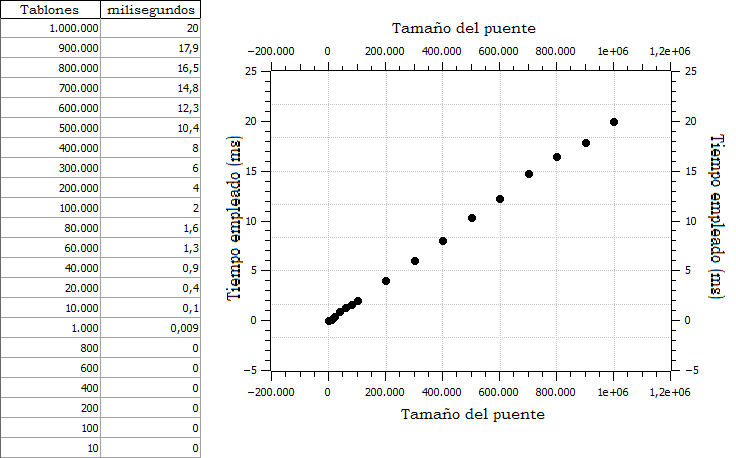
\includegraphics[scale=0.75]{casosDeTest/GRAFICOS/png/Ej1peorCasoPNG.png}
		\end{center}
	\end{figure}

En la figura superior se puede apreciar que el tiempo de resolución de peor caso del algoritmo es lineal al tamaño del puente de entrada.

\subsubsection{Escenarios de casos promedio del algoritmo}

\noindent En estos escenarios, decidimos evaluar y tomar métricas para casos no tan “border”  como los de los escenarios anteriores. La idea es tomar muestras del algoritmo haciendo variar la longitud de salto del participante como el tamaño del puente, generando de manera aleatoria el estado de los tablones del mismo.

\noindent Para diferenciar bien los casos y poder analizar mejor, decidimos que cada escenario de las pruebas de caso promedio tenga una capacidad de salto constante. En cada uno de estos escenarios veremos cómo responde el algoritmo a medida que varía el tamaño de la entrada.

\noindent Notar que a diferencia  del mejor y del peor caso, aquí no está garantizado que el participante vaya a cruzar todo el puente. En los casos anteriores, cruzar el puente era requerido para poder contemplar el caso de análisis, tanto para el mejor como para el peor caso. Para poder ver en los gráficos, no solo el tiempo de respuesta del algoritmo en función de la entrada, sino también si el participante pudo o no cruzar el puente, se marcó de color verde a las instancias en las que sí pudo, y de color rojo a las que no.

\noindent Como era de esperar, como el estado de cada tablón es aleatorio, mientras más pequeño es el salto del participante, mayor es la probabilidad de que este no pueda cruzar el puente, ya que la probabilidad de que haya tantos tablones inválidos consecutivos como la capacidad de salto, aumenta.

\noindent Dicha probabilidad también aumenta cuando el puente crece, ya que hay un mayor espacio para que dicha secuencia de tablones inválidos aparezca.

\noindent Como fue mencionado anteriormente, para realizar estas pruebas, se diseñó un generador de instancias de caso promedio, que dado un tamaño de entrada y una capacidad de salto, generaba tantas instancias distintas como se quisiera, respetando el tamaño asignado. Eso nos permitió evaluar la respuesta del algoritmo para distintas instancias del mismo tamaño, y poder tomar un promedio.

\noindent Para estos casos, también cada prueba de cada escenario fue repetida un total de 10.000 veces para aminorizar el margen de error producido debido a que el CPU no está atendiendo únicamente nuestro proceso.

\noindent Como última observación a hacer, es interesante notar que para los casos en los que el participante no pueda cruzar todo el puente, los tiempos no siguen ningún patrón ni concordancia, ya que, si llamamos C a la capacidad de salto de un participante, el hecho de que haya C tablones rotos consecutivos es totalmente aleatorio ya que el estado de los tablones fue generado de manera aleatoria.

\noindent Sin más, presentamos los distintos escenarios.\\

\newpage \indent ESCENARIO DE SALTO = 2

	\begin{figure}[h]
		\begin{center}
		   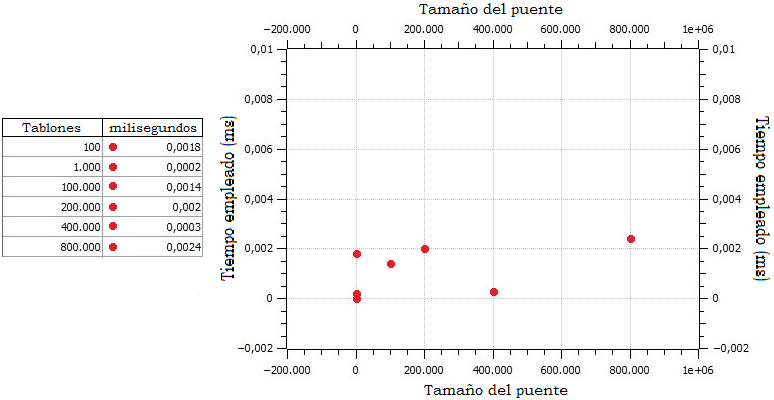
\includegraphics[scale=0.75]{casosDeTest/GRAFICOS/png/randoms/ej1_random_salto2.png}
		\end{center}
	\end{figure}

Tal como lo expresado anteriormente, para saltos de baja longitud, la probabilidad de no poder cruzar el puente aumenta, por lo que los tiempos del algoritmo pueden variar mucho de instancia a instancia. \\ \\

\indent ESCENARIO DE SALTO = 4
	\begin{figure}[h]
		\begin{center}
		   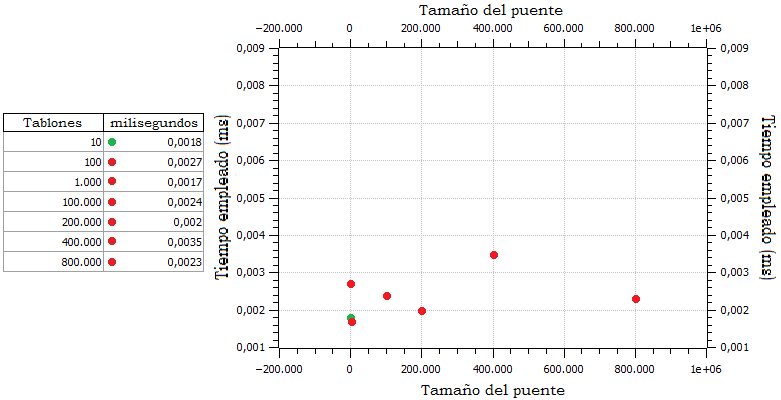
\includegraphics[scale=0.75]{casosDeTest/GRAFICOS/png/randoms/ej1_random_salto4.png}
		\end{center}
	\end{figure}

Aquí se puede apreciar que una de las instancias generadas permitió al participante cruzar todo el puente, y que fue la instancia en la que más probabilidades tenía de hacerlo, es decir, la instancia con un puente de longitud = 10. Para el resto, continuaron apareciendo de manera aleatoria distintos baches en el puente que no permitieron al jugador terminar de cruzar el mismo. Notar que los baches se hicieron presentes al poco tiempo de recorrer el puente, tal como era esperado probabilísticamente.\\

\newpage \indent ESCENARIO DE SALTO = 8
	\begin{figure}[h]
		\begin{center}
		   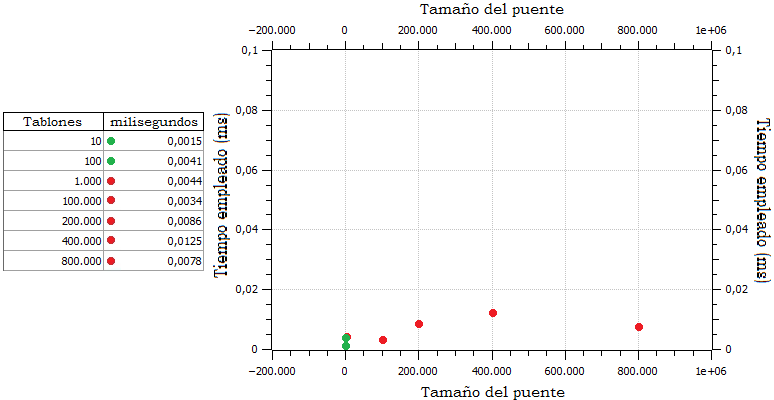
\includegraphics[scale=0.75]{casosDeTest/GRAFICOS/png/randoms/ej1_random_salto8.png}
		\end{center}
	\end{figure}

En saltos de tamaño 8, se continuó observando que la probabilidad de poder cruzar el puente en altas instancias continúa siendo muy baja y el algoritmo termina rápidamente debido a eso.  Aunque como cada instancia no depende de las demás, no podemos acotar al tiempo del algoritmo, pero si podemos hacerlo, justificando que cierta cota es válida para el caso promedio, para saltos menores o iguales a 8.\\

\indent ESCENARIO DE SALTO = 16
	\begin{figure}[h]
		\begin{center}
		   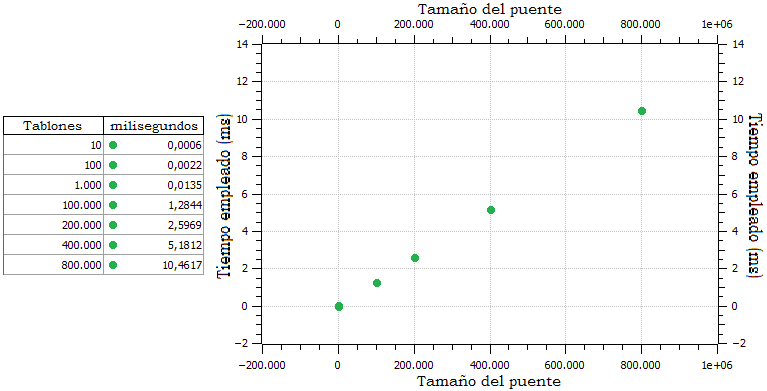
\includegraphics[scale=0.75]{casosDeTest/GRAFICOS/png/randoms/ej1_random_salto16.png}
		\end{center}
	\end{figure}

A partir de aquí, notamos que con las mismas longitudes de prueba que en los escenarios anteriores, no se produjo una caída del puente, en ninguna de las distintas instancias que se probaron para cada uno de los tamaños (10, 100,…,800.000). Vale destacar, que con un salto de longitud = 16, se cae en el mejor caso, para la instancia de 10 tablones, ya que puede cruzarla toda de una, haciendo que la probabilidad de caer del puente pase a ser nula. Lo mismo ocurrirá con luego con saltos mayores, al superar a la instancia de 100 tablones.

Si bien en todas las pruebas de este escenario el participante pudo cruzar, eso no escapa de la probabilidad de que la generación aleatoria pueda dar 16 tablones rotos consecutivos. Por lo que no podemos dar una cota fija, pero podríamos estimar que en el caso promedio, el puente puede ser cruzado, lo que da una complejidad de O(n) para el caso promedio, con n igual a la cantidad de tablones.
Es O(n) ya que el algoritmo debe recorrer todo el puente para terminar.\\

\newpage \indent ESCENARIO DE SALTO = 32
	\begin{figure}[h]
		\begin{center}
		   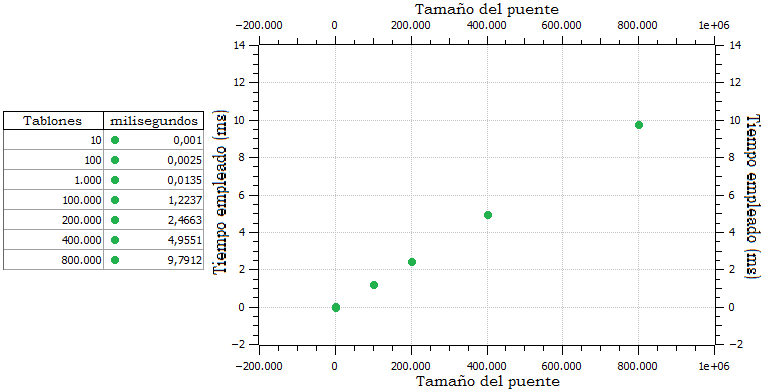
\includegraphics[scale=0.75]{casosDeTest/GRAFICOS/png/randoms/ej1_random_salto32.png}
		\end{center}
	\end{figure}

Aquí y en adelante, la probabilidad de que haya una cantidad de tablones rotos consecutivos igual a la cantidad del salto, es realmente baja, más allá del tamaño de la entrada; tendría que ser una entrada exageradamente grande para que la probabilidad aumente apenas un poco. Por ende de aquí en adelante, afirmamos que el caso promedio del algoritmo es O(n), (recordando que n es la cantidad de tablones del puente en cuestión).

Por lo dicho recién, en los siguientes escenarios era esperado que la respuesta del algoritmo sea líneal al tamaño de la entrada.\\ \\

\indent ESCENARIO DE SALTO = 64
	\begin{figure}[h]
		\begin{center}
		   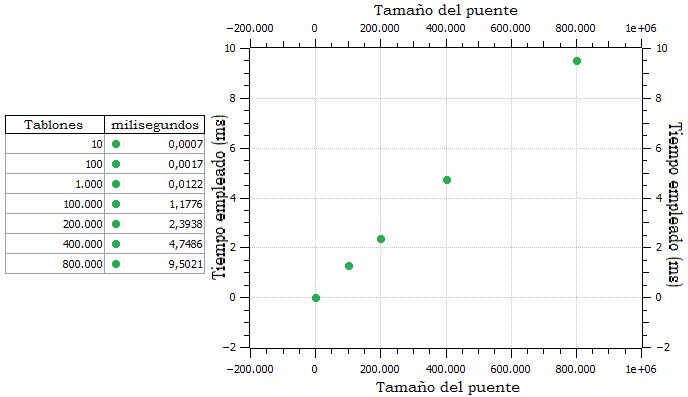
\includegraphics[scale=0.90]{casosDeTest/GRAFICOS/png/randoms/ej1_random_salto64.png}
		\end{center}
	\end{figure}

\newpage \indent ESCENARIO DE SALTO = 128
	\begin{figure}[h]
		\begin{center}
		   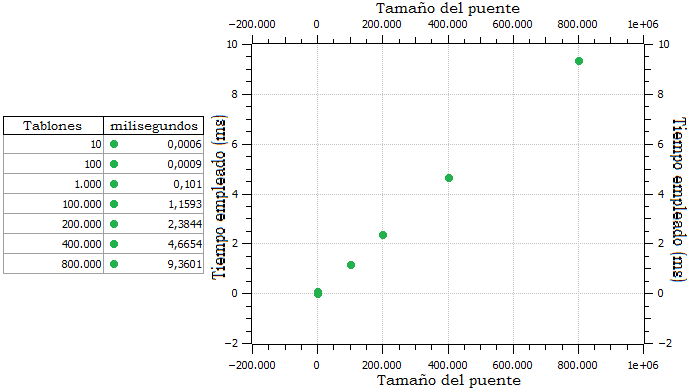
\includegraphics[scale=0.90]{casosDeTest/GRAFICOS/png/randoms/ej1_random_salto128.png}
		\end{center}
	\end{figure}

\indent ESCENARIO DE SALTO = 256
	\begin{figure}[h]
		\begin{center}
		   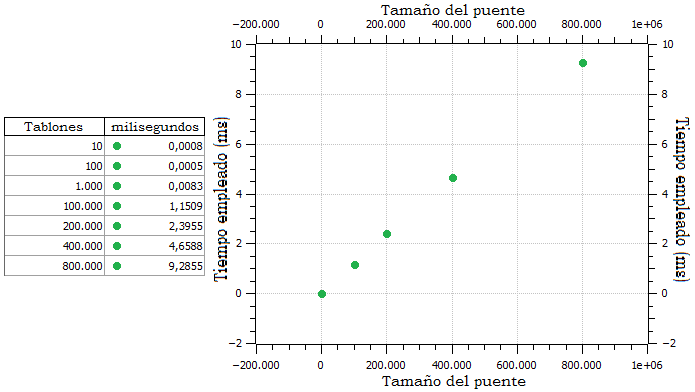
\includegraphics[scale=0.90]{casosDeTest/GRAFICOS/png/randoms/ej1_random_salto256.png}
		\end{center}
	\end{figure}


\subsubsection{Algunas conclusiones}
Haciendo un análisis probabilístico de nuestro algoritmo, por lo antes explicado podemos afirmar que en saltos grandes, el tiempo de computo de una instancia es lineal al tamaño del puente de la misma.
En cuanto a saltos pequeños no hay un patrón que se mantenga ya que el “hueco” sin tablones válidos por los cuales no se podría cruzar es totalmente al azar, pero probabilísticamente, si el salto es chico, dicho “hueco” se hará presente al poco tiempo de computo, por lo que el algoritmo responde eficientemente y podríamos acotar este tiempo para un caso promedio.

\end{document}